\documentclass[conference]{IEEEtran}

\usepackage{graphicx,times,psfig,amsmath,url,multirow,color,soul}
\usepackage{epstopdf}
\usepackage{subfig}

%\usepackage{epstopdf}
%\usepackage[scientific-notation=true]{siunitx}

\hyphenation{}

\DeclareRobustCommand{\hlcyan}[1]{{\sethlcolor{cyan}\hl{#1}}}

\begin{document}

\title{Sensory Configurations for Collective Behavior}

\author{}

%\author{\IEEEauthorblockN{James Watson}
%\IEEEauthorblockA{jwatson@cs.uct.ac.za}
%\and
%\IEEEauthorblockN{Geoff Nitschke}
%\IEEEauthorblockA{gnitschke@cs.uct.ac.za}}

\maketitle

\begin{abstract}
This paper presents a study on the impact of different robot sensory
configurations (morphologies) 
in simulated robot teams that must accomplish a
collective (cooperative) behavior task. 
The study's objective was to investigate if effective collective 
behaviors could be efficiently evolved given minimal morphological 
complexity of individual robots in a homogenous team.
A range of sensory configurations are tested in company with evolved controllers
for a collective construction task.
Results indicate that a minimal sensory configuration yields the
highest task performance, and increasing the complexity of the sensory
configuration does not yield an increased task performance.
\end{abstract}

%This research uses a collective gathering task where task complexity is moderated via
%requiring varying degrees of cooperation to complete the task.



\IEEEpeerreviewmaketitle

\section{Introduction}

An open problem in \textit{cooperative multi-robot systems} \cite{Farinelli2004}
is determining, \textit{a priori} the most appropriate sensory-motor configuration (morphology)
for individual robots, such that when an automated controller design (behavioral adaptation)
method is applied, a robot team evolves a collective behavior to solve a given cooperative 
task.

This study falls within \textit{Evolutionary Robotics} (ER) \cite{NolfiFloreano2000} research
within the larger taxonomy of cooperative multi-robot systems \cite{Farinelli2004},
where \textit{Neuro-Evolution} (NE) \cite{FloreanoDurrMattiussi2008} is used to evolve controllers
for a morphologically homogenous team.
A popular approach in ER is to
employ \textit{Cooperative Co-Evolutionary Algorithms} (CCAs) \cite{GomezMiikkulainen1999},
\cite{PotterDeJong2000}, \cite{WiegandLilesDeJong2001} to co-adapt robot behaviors and morphologies.
Such approaches have been successful for finding robot morphologies and controllers specifically
suited to accomplishing various tasks and in a range of environments \cite{Sims1994},
\cite{MautnerBelew2000},
\cite{LipsonPollack2000},
\cite{HornbyPollack2001b},
\cite{HornbyPollack2002},
\cite{Lund2003},
\cite{BongardPfeifer2003},
\cite{BuasonBergfeldtZiemke2005},
\cite{AuerbachBongard2014}.
%\cite{LundLee1997},
%\cite{AdamatzkyUlatowski2000},
%\cite{HornbyPollack2001},
%\cite{Eggenberger1997},
%\cite{AuerbachBongard2010},
%\cite{CheneyLipson2013},
%\cite{BuasonZiemke2003},
%\cite{SchultzBugajska2003},

%This is especially the case for collective behavior tasks  \cite{PfeiferBongard2006}, \cite{TruebaDuro2011}.
However, due to the computational complexity and intractable search spaces there has been relatively little
research on the co-evolution of morphology and behavior, excluding self-assembly \cite{OGradyDorigo2012} 
in multi-robot \cite{AsaiArita2003} and swarm robotic \cite{Beni2004} systems.
An alternate approach to using CCAs in ER multi-robot systems is to systematically test a range of robot
morphologies in company with controller evolution, in order to ascertain the best team morphology and
behavior for a given task and environment.
For morphologically homogeneous teams such an approach does not entail intractable search spaces or exponentially
increasing computational complexity of increasing team sizes and task complexity.
Rather, the experimenter must design a set of \textit{morphological parameter tuning} experiments that
test a sufficiently diverse yet functional range of robot morphologies.  In this case some \textit{a priori}
knowledge of the task is assumed.

\hlcyan{For the hilighted text below, should change it to "The objective of this research is to determine the robustness of controllers evolved using HyperNEAT with regards to their changing sensory configuration"}

\hl{This study's research objective was to ascertain the most appropriate morphology for a homogeneous robot team,
that enables the team to efficiently evolve an effective team behavior that solves a collective behaviour
task.}  The task was collective construction, where cooperation was required for robots to gather
and connect (build a structure) from all resources (blocks) in an environment.
Each robot in the team has the same morphology, and an \textit{Artificial Neural Network}
(ANN) controller with a variable number of sensory inputs and hidden layer nodes and 
a fixed number of motor outputs.

Whilst the number of sensory input and hidden nodes and sensor ranges were determined by the experimenter, 
the ANN connection weights and inter-layer connectivity was adapted with HyperNEAT
\cite{StanleyDAmbrosioGauci2009}.  Teams were behaviorally homogeneous in that the current 
fittest ANN controller was copied \textit{P} times for \textit{P} robots in a team.  
Each robot also used the same morphology.
HyperNEAT was selected as it has been successfully applied to evolve team behaviors for various tasks
including \textit{RoboCup} \cite{verbancsics_evolving_2010} and multi-agent
\textit{Pursuit-Evasion} \cite{DAmbrosioStanley2008}.  Also, HyperNEAT is a generative encoding method,
and such methods have been demonstrated as beneficial as they tend to produce regular and modular
ANNs with increased learning capacities \cite{TonelliMouret2013}.
%A homogenous team (all robots have the same morphology and behavior) was selected to bypass the credit assignment problem \cite{HaynesSen1996B}
%and to focus on the role of varying team morphologies, versus collective gathering task complexity.
%is chosen as the method through which the ANN is generated. The parameters to be optimised will be restricted to the number of sensors and their detection range. HyperNEAT has been used  in a wide variety of cooperative tasks including a predator prey scenario \cite{dambrosio_generative_2008}, and both the RoboCup keep-away and RoboCup soccer benchmarks \cite{verbancsics_evolving_2010}.

In this study, a \textit{collective construction} task \cite{Werfel2007}, which was a variation of 
\textit{collective gathering} \cite{BonabeauDorigo1998} was selected.  
The task was for robots to search for randomly distributed resources (blocks) in the environment and
then move them such that they connected to other blocks in the environment, where the goal was for
all blocks to be connected.

\hlcyan{For the highlighted text below: "In this instance of the collective construction task, three different block types were used. The first can be moved by a single robot while the second and third type require two and three robots to move them respectively."}  
\hl{One block type required cooperation between robots to move, while another could be moved by individual robots. } 

\hlcyan{For the highlighted text below: "In this case, the complexity of the basic task is increased/controlled/manipulated using a construction schema, which is a collection of underlying connection rules that specify which type of block can be connected to another block as well as on which side. (do not have a target structure to be built)}

\hl{In this case, blocks could be connected to any other in order that a structure be built. 
However, this is a simplified version of a 
more complex construction task that requires robots to collectively build a structure via connecting resources
in specific ways such that a target structure is built} \cite{WerfelPetersenNagpal2014}.

Potential future applications of finding effective solutions to such a task 
include construction for exploration and mining in hazardous and remote
environments \cite{BrooksMaesMataricMore1990}, \cite{ShenKhoshnevis2003}, where functional structures and habitats
must be built from a set of prefabricated modules without human direction
\cite{WerfelBarYamNagpal2005}, \cite{WerfelNagpal2008}.
%This study only addresses the collective gathering sub-task, and current research is addressing
%the collective construction task.%\cite{NitschkeSaEC2012}.
%In this study's collective gathering task, division of labor is required given that varying degrees of
%cooperation are required to move different resource types, and maximize resources
%gathered. Thus the collective gathering task is modeled as an optimization problem
%\cite{BonabeauTheraulaz1996} and optimal solutions are attainable with evolutionary
%approaches \cite{WaibelFloreano2006}.

This study is a preliminary step in producing NE methods that autonomously adapt multi-robot and
swarm robotic system behaviors and morphologies such that problem solving collective behaviors
are produced for high level user specified goals \cite{JonesMataric2003}.
This relates to recent research in \textit{collective gathering} and
\textit{construction} \cite{WerfelPetersenNagpal2014}
and \textit{self-assembly} \cite{RubensteinCornejoNagpal2014}, where desired structures are specified by a user
and robots adapt their individual behaviours in order to collectively build or self-assemble a desired structure.

\subsection{Collective Construction Task:} \label{subsec:constructionTask}
This task requires a simulated robot team to gather blocks and
cooperatively build a structure from gathered blocks in a
bounded continuous environment (figure \ref{fig:env}).

\hlcyan{For the highlighted text below: "The complexity of this task is equated with the degree of cooperation (number of robots required) to collectively transport blocks and connect them together with other blocks in order to build a structure (resultant from connecting all blocks in the environment) as well as the difficulty of the implemented construction rules that determine how the blocks can be connected to each other."}
\hl{The complexity of this task is equated with the degree of cooperation
(number of robots required) to collectively transport blocks and connect
them together with other blocks in order to build a structure
(resultant from connecting all blocks in the environment).}

\hlcyan{For the text below: "In this research there are three block types, \textit{A}, \textit{B} and \textit{C} that require one, two and three robots to transport, respectively."}
\hl{In this research there are two block types, \textit{A} and \textit{B} that require one and two robots to transport, respectively.}


The blocks must be connected into a structure according to a
\textit{construction schema}, that dictates the sequence for how 
block types must be connected.

\hl{However, for the testing purposes of this preliminary research the construction schema allows blocks to be connected together in any sequence.} 

\hlcyan{For the highlighted text above: "The construction schema and the different block types are used to implement four levels of complexity with which the controllers are tested. These complexity levels consist of various combinations of block types and construction schema as follows:"}

\begin{itemize}
	\item Level 1: no complexity and no cooperation required. Each of the block types present in the simulation can be connected to any of the other block types (no complexity) and each block can be moved by a single robot (no cooperation).
	\item Level 2: no complexity and some cooperation. Each of the block types can be connected to every other block type (no complexity) but each type can only be moved by its respective number of robots (some cooperation).
	\item Level 3: some complexity and no cooperation. This means there are some relatively simple connection rules in the construction schema (some complexity) but each type of block can still be moved by a single robot.
	\item Level 4: complexity and cooperation required. For this level, the most difficult construction schema is implemented and each of the block types can only be moved by its respective required number of robots.
\end{itemize}

\hlcyan{It should also be noted that when two previously free blocks are connected, they form a construction zone. Other blocks in the environment can then only be connected to a construction zone.}

Task performance (team fitness) is the number of blocks connected
(as a built structure) during a team's lifetime 
(table \ref{tab:simParameters}).

\begin{figure}[t]
    \centering
    \includegraphics[width=0.4\textwidth]{NewGraphics/Simulator.png}
    \caption{\hlcyan{Collective Construction Task Example In Simulator:
    Robots are the black squares with white arrows indicating the direction they are facing. The blocks are the blue, green and red squares indicating type A, B and C, respectively.
    The construction zones are indicated by the blocks with their respective type labels. These are the structures that have been built thus far.
    The translucent coloured sectors indicate the range and field of view of the sensors currently equipped to the robots.}
    \hl{Collective Construction Task Example:
    Robots are the circles and blocks as the small (\textit{Type A}) and large (\textit{Type B}) rectangles.
    The green structure is that which has been built thus far via robots pushing blocks together.}}
   \label{fig:env}
\end{figure}

%\section{Collective Gathering Task}
%To measure the effect of changing the configuration of agents' sensors, a simpler gathering subtask was used.
%The collective construction task required group of simulated robots with randomized starting positions surrounded by blocks,
%the goal being for robots to be distributed amongst the blocks such that each block received either one or two robots
%depending on its randomly chosen type.
%Performance was measured by the number of agents successfully assigned to blocks, and the number of blocks receiving their maximum number of agents.
%The task environment consists of a rectangular bounded area (100 by 100 units), a group of robots, and a group of blocks.
%Robots start near the center of the world with randomized starting positions and rotations, and blocks surround them, also with randomized positions.
%When evaluating a given genotype multiple times to average the resulting fitness the same starting layout is used, but different layouts are generated for each new genotype. Blocks have a capacity (the number of agents required before it can be moved) of either 1 or 2 robots.
%The task environment consists of a rectangular bounded area measuring , a group of agents, and a group of blocks. Agents start near the centre of the world with randomised starting positions and rotations, and blocks surround them - also with randomised positions.  When evaluating a given genotype multiple times to average the resulting fitness the same starting layout is used, but different layouts are generated for each new genotype. Blocks have a capacity (the number of agents required before it can be moved) of either 1 or 2 agents.

%The collective construction task studied in this article, requires that agents first gather resources and place
%them in a construction zone.  Collective gathering tasks require that agents search for, and transport resources
%from given locations to another part of the environment \cite{BonabeauDorigo1998}.
%There are numerous examples of adaptive methods applied to simulated agent groups
%in order that collective gathering \cite{Thangavelautham2008}, \cite{EibenKarafotiasHaasdijk2010}, \cite{NitschkeKrevelen2008},
%\cite{MurcianoMillan1997}, \cite{IjspeertMartinoli2001}, \cite{WaibelFloreano2006},
%\cite{GautraisTheraulaz2002}, \cite{BonabeauSobkowski1997} or construction \cite{TheraulazBonabeau1995},
%\cite{ThomasHowardWilliamsMooreAlston2005}, \cite{GuoMengJin2009b}, \cite{WerfelNagpal2008}, \cite{PanangadanDyer2009}
%tasks are solved.

%In using neuro-evolution for multi-agent simulations, past research generally has either introduced new methods, or compared the performance of various methods. Examples of this include the papers introducing NEAT \cite{stanley_efficient_2004}, SANE \cite{moriarty_efficient_1996} (and subsequently ESP \cite{gomez_robust_2003}), and CMA-ES \cite{hansen_completely_2001}. These all relied on direct encodings and homogeneous designs. One innovation seen in similar research is indirect encoding, as in HyperNEAT \cite{stanley_hypercube-based_2009} \cite{gauci_autonomous_2010}, EANT \cite{kassahun_efficient_2005}, and EANT2 \cite{siebel_evolutionary_2007}. Another is the introduction of heterogeneous versions of existing methods, allowing for teams of agents to adapt to different roles, including multi-agent HyperNEAT \cite{dambrosio_evolving_2010} \cite{dambrosio_generative_2008} and multi-component ESP \cite{miikkulainen_multiagent_2012}.
%This paper will look at another aspect of the problem, namely how to use the results of the simulation to guide the design of agents, as opposed to using an arbitrarily chosen agent design and maximising its performance. This could allow for more efficient physical implementations of such tasks in terms of both costs and time taken.
%The approach taken in this paper is to use neuro-evolution to generate artificial neural networks (ANNs),
%which when given an agent's sensory input will determine the action it takes. Neuro-evolution requires the ability to evaluate potential solutions many times, which is made possible using a simulation. The final neuro-evolution implementation will also be able to solve a wide variety of problems without the need for hard-coding details, such as different target layouts of the structure, number of agents, environmental constraints.
%This research addresses a sub-set of the collective construction task, where a simulated robot team must collectively (cooperatively) gather resources
%distributed throughout an environment and transport them to a home area (construction zone).
% such as autonomous construction of a lunar base
%Agents detect sensory input from the environment
%and adjust their movement using some controller. The problem to solve is then the generation of an appropriate controller.
%test a range of team morphologies in company with controller evolution
%for a collective behavior (gathering) task of varying complexity.
%co-adapt the sensory configurations and controllers of individual robots such that
%collective behaviour tasks are cooperatively solved.
%uses Neuro-Evolution
%comparative studies of generative NE methods
%in the context of simulated cooperative multi-robot systems.
%Whilst there has been a significant amount of work in ER that focuses on the co-evolution of behaviour and morphology
%With this approach body plans and control policies uniquely suited for a machine�s task environment may be found.
%Multi-agent simulations allow us to observe the behaviour of a group of agents, without the need for a physical implementation.
%In particular, when the individual agents are autonomous robots a simulation would drastically reduce the cost and time needed to run experiments.
%One such multi-agent scenario is the collective construction task, in which a group of agents must build a structure by moving ``blocks'' around the environment until a predetermined target layout is achieved.

\section{Methods}

HyperNEAT \cite{StanleyDAmbrosioGauci2009} is an extension of the NEAT (\textit{Neuro-Evolution of Augmented Topologies})
\cite{Stanley2004} method, where ANNs are indirectly encoded using a CPPN (\textit{Compositional Pattern Producing Network})
\cite{Stanley2007}.  
In this case, HyperNEAT evolves the connection weights and the connectivity between a fixed sensory input layer, 
hidden layer and motor output layer.
HyperNEAT was selected since geometric features in the task environment, are exploited during controller evolution.
In the collective construction task, such geometric feature include the relative positions of other robots, blocks,
and the direction robots and blocks are facing.  
HyperNEAT has also been demonstrated as being capable of exploiting regularity and
modularity in multi-agent tasks in order to evolve solutions that could not otherwise be evolved \cite{DAmbrosioStanley2008}.
In the collective construction task, HyperNEAT is potentially beneficial, given that structures to be built are modular
(comprised of a set of blocks), and regular (the same sequence of blocks can be repeated).

\begin{figure*}[t]
    \centering
    \includegraphics[width=0.5\textwidth]{NewGraphics/Morphology.png}
    \caption{ \hlcyan{Example robot sensory configuration indicating the relative positions of various sensors on the robot}}
    \label{fig:Morph}
\end{figure*}

\begin{figure*}[t]
    \centering
    \begin{minipage}{0.23\textwidth}
       	\centering
        \includegraphics[width=\textwidth]{necc_paper_ann_i.eps}
    \end{minipage}
    \begin{minipage}{0.23\textwidth}
        \centering
        \includegraphics[width=\textwidth]{necc_paper_ann_i.eps}
    \end{minipage}
    \begin{minipage}{0.23\textwidth}
        \centering
        \includegraphics[width=\textwidth]{necc_paper_ann_o.eps}
    \end{minipage}
    \caption{ANN Topology as it relates to robot morphology: Sensory input layer (left), hidden layer (center) and motor output layer (right).
    Output nodes \textit{R} and \textit{S} determine a robot's rotation and speed, respectively.
    Arrows indicate the direction the agent is facing.}
    \label{fig:ann}
\end{figure*}

\hlcyan{not sure of the figure showing the ANN topology. We just created the same number of input nodes as there are sensors, not sure if the geometry is matched in the way that they illustrate. Also, the outputs for our ANN's map to the left and right wheel, the output value being how fast that wheel must rotate}

%\vspace{-0.4cm}
\subsection{Robot Controller}\label{sec:embodiment}
%\vspace{-0.2cm}
All robots in a team used the same ANN controller, where each controller had
\textit{N} sensory input nodes (determined by a given experiment set), that
adaptively mapped sensory inputs, via a hidden layer, to two motor outputs
(figure \ref{fig:ann}) using HyperNEAT \cite{StanleyDAmbrosioGauci2009}.

Figure \ref{fig:ann} illustrates an example ANN configuration for \textit{N} = 6.
The ANN uses a 3 dimensional coordinate system for processing \textit{x}, \textit{y}, \textit{z}
positions in the CPPN in order to generate weight and bias values and connectivity.
The CPPN indirect encoding of HyperNEAT allows evolved controllers to exploit the geometry
of the task and the environment.

Also, HyperNEAT exploits the configuration of nodes in the ANN controller, thus the sensory input and motor output nodes
must be in an appropriate configuration reflecting their position as part of a robot's morphology.
Nodes for processing sensory inputs correspond to the direction each sensor faces.
Thus, the input layer of the ANN controller is a circle of \textit{N} evenly distributed nodes.

\hlcyan{For the text below: The FOV of each equipped sensor is shown in the image, they do not make a complete 360 degree FOV, not sure if this is relevant}
\hl{Each node is a sensor, where the sensory \textit{Field of View} (FOV) of all sensors forms a complete 360 degree
FOV} (figure \ref{fig:Morph}).

\hlcyan{For the text below: The output nodes correspond to the left and right wheel actuators, producing an output [-1.0, 1.0] that indicates how fast each respective wheel must turn. Equal output means straight forward motion and unequal output results in the robot rotating about its own axis.}

\hl{The rotation output node is in the center to
preserve the angle between sensory input nodes.
The speed output node is offset in the direction the
robot is facing to signify forward movement at a given speed.}

\hlcyan{while they keep mentioning that the output is mapped to a rotation and speed node, later on in the section titled Movement Actuators, they talk about how the output is mapped to the left and right wheels. Not sure if this is an inconsistency or I am misunderstanding something}


The intermediate hidden layer reflects the configuration of the input layer, in order
to preserve the geometry of the sensory input layer, that is the direction of each sensor's FOV (figure
\ref{fig:ann}).
The ANN is initialized with full connectivity between adjacent layers, however, partial connectivity 
can be evolved via
the CPPN generating a zero weight.
During the neuro-evolution process, the CPPN is developed via having nodes and connections added and removed, as well
as connection weight values mutated \cite{StanleyDAmbrosioGauci2009}.  Neuro-evolution parameters used in this
study are given in table \ref{tab:NEParameters}.

\hlcyan{The subsubsection below called Block Detection Sensors is the original content from the paper. The subsubsection below that called Detection Sensors is the content that I added/changed}

\subsubsection{Block Detection Sensors}
Each robot has \textit{N block detection} sensors each with a range of \textit{r} (portion of the environment's length). Given that \textit{N} and \textit{r} are the subject of the experimental comparisons of this research, they are determined by the experimenter \ref{sec:experiments}. Robots are unable to detect each other , thus all cooperative interactions are \textit{stigmergic} \cite{BeckersHollandDeneubourg1994}, taking place via the blocks and the built structure in the environment. A robot's 360 degree sensory FOV is split into \textit{N} sensor quadrants \ref{fig:Morph}. Block detection sensors are constantly active for the duration of the robot's lifetime. Sensor \textit{q} returns either 0 (no blocks detected) or 1 (one or more blocks detected) in sensor quadrant \textit{q}. All detection sensor values are normalized within the range [0.0, 1.0].

\subsubsection{Detection Sensors}
As shown in \ref{fig:Morph}, each robot is equipped with a variety of different types of abstracted sensors so as to simulate the different types of sensors that might be used in the real world. Each sensor has a specified field of view (FOV), range and bearing (its relative position on the robot) that is predetermined by the experimenter. While the range and FOV of the sensor remains constant, its bearing changes depending  on the sensory configuration that the robot is equipped with. The range and FOV of each type of sensor is shown in table \ref{tab:NEParameters}.


\begin{table} 
	\centering
	\caption{A table showing the different types of sensors used in the experiments in the left column and the right column shows the sensory configuration (morphology number) that they are part of. The second set of numbers in parentheses indicate the number of that sensor present in each respective morphology listed before.}\label{tab:morphsPerSensor}
	\begin{tabular}{| c | c |}
		\hline
		Sensor Type		& 		Morphology Number \\ \hline
		Proximity		&		1,2,4,5,6,7 (5,4,2,2,5,5)	\\
		Ultrasonic		&		1,2,5,6,7 (3,1,2,3,3)		\\
		Colour Ranged	&  		1,2,3,4,5,7 (1,1,1,1,1,1)   \\
		Low-Res Camera	&		1,2,3,4,5 (1,1,1,1,1)		\\
		Construction  	&		1,2,3,4,5,6,7 (1,1,1,1,1,1,1) \\ 
		\hline
	\end{tabular}
\end{table}


Each robot has \textit{N} sensors each with a specified range, field of view and bearing (its position on the robot). The subject of these experimental comparisons is the various combinations of these different types of sensors (referred to as sensor morphologies) that are implemented in the different experiments. These sensor morphologies are predetermined by the experimenter and are outlined later on in this table. Robots are unable to detect each other, thus all cooperative interactions are
\textit{stigmergic} \cite{BeckersHollandDeneubourg1994}, 
All detection sensor values are normalized within the range [0.0, 1.0].

\subsubsection{Movement Actuators}

\hlcyan{not sure about this section because the output nodes map to left and right wheels and not to rotation and speed nodes}

Two motor outputs control a robot's heading and speed (\textit{R} and \textit{S} in figure \ref{fig:ann}) of
movement.
Motor output values are normalized within the range [-1.0, 1.0], where \textit{R}, \textit{S} = 0.0 corresponds to
a default heading and being stationary, for the rotation and speed motors, respectively.
Negative values of \textit{R} and \textit{S} correspond to anti-clockwise rotation and decreasing speed, where as,
positive values correspond to clockwise rotation and increasing speed.
\textit{R} values of -1.0 and 1.0 equate to keeping the same heading, and an \textit{S} value of 1.0 equates to
the maximum distance a robot can traverse in one simulation iteration ($MaxDistance$ in table \ref{tab:simParameters}).

\section{Experiments}\label{sec:experiments}

Experiments test \textit{n} robots in a bounded two dimensional continuous environment (20 x 20 units) containing a random distribution of type \textit{A}, \textit{B} and \textit{C} blocks
(table \ref{tab:simParameters}).  Robots are randomly initialized in the
environment.


Figure \ref{fig:env} illustrates an example environment, \hlcyan{containing 15 robots and 15 blocks of type} \textit{A}, \textit{B} and \textit{C}.


Figure \ref{fig:env} illustrates an example environment, \hl{containing 30 robots and 10}
\textit{type A} and \textit{B} blocks.

How different block types are connected is dictated by a \textit{construction schema}
defining the sequence of block types that must be connected together in order for a
structure to be built.  



\hlcyan{should possibly remove the highlighted text below. Or say: "Since the preliminary studies have been done, this investigation will implement the various connection rules that are illustrated in figure} \ref{fig:constructionSchema}

\hl{However, since this is a preliminary study to demonstrate a simple collective construction task, blocks can be connected in any sequence.}

\begin{figure}[t]
	\centering
	\includegraphics[width=0.5\textwidth]{NewGraphics/ConstructionSchema.png}
	\caption{An example of the various connection rules implemented in this experiment's construction schema. \hlcyan{This is an old image, still need to create one for this years experiments}}
	\label{fig:constructionSchema}
\end{figure}

The difficulty of the construction task is regulated via requiring varying degrees of
cooperation to make specific block connections.
In this task, cooperation refers to at least two robots simultaneously gripping and
pushing a block to touch another block, to which it automatically connects.

\hlcyan{Once two previously free blocks are connected for the first time, a construction zone is formed. A construction zone refers to any structure that has been built in the environment. Once a construction zone is created, all resources that get attached to it are fixed in position and can not be disconnected again. There are only allowed to be three construction zones at a time and free blocks can only be connected to existing construction zones.}

One robot only is required to push type \textit{A} blocks, two robots are needed to push
type \textit{B} blocks and three robots are needed to push type \textit{C} blocks.

\subsection{Experiment Design}\label{subsec:expDesign}

\hlcyan{For the highlighted text below: "These experiments determine the robustness of HyperNEAT evolved multi-robot controllers with regards to completing the collective construction task given a varying sensor morphology}

OR 

\hlcyan{Experiments measure the ability of HyperNEAT evolved controllers to complete the collective construction task of varying complexity given changes in its sensory configuration}


\hl{Experiments measure the impact of varying robot morphology
upon the evolved group behavior of a homogeneous robot team given a collective construction
task and a simulation environment.}

\hlcyan{For the highlighted text below: "The collective construction task requires robots to search the environment for blocks and then push the blocks connecting them to other construction zones in the environment, in order to build a structure."}

\hl{The collective construction task requires robots to search the environment for blocks and then push the blocks connecting them to others in the environment in order to build a structure.}

Team task performance equals the number of blocks connected
together during a team's lifetime (equation \ref{equ:FitnessFunction}).  
An environment is defined as a distribution
of block types, robots, and a construction schema.

\hlcyan{For the highlighted text below: "To investigate the behavioural robustness of multi-robot team controllers evolved using the HyperNEAT algorithm with respect to sensory configurations when implemented in solving increasingly complex tasks requiring collective behaviour."}

\begin{table}
	\renewcommand{\arraystretch}{1.3}
	\caption{Sensor, Experiment and Neuro-evolution Parameters}\label{tab:NEParameters}
	\centering
	\begin{tabular}{llc}
		\hline
		Generations	                         & 100	\\
		Sensors per robot                    & 11, 8, 4, 6, random \\	
		Evaluations per genotype             & 5  \\
		Experiment runs                      & 20 \\
		Environment length, width            & 20 \\
		MaxDistance                          & 1 \\
		Team size                            & 15 \\
		Team Lifetime (Task scenario length) & 1000 \\	
		Lifetimes per generation             & 5 \\   
		Type A blocks (1 robot to push)      & 15, 5, 5 \\
		Type B blocks (2 robots to push)     & 0, 5, 5 \\
		Type C blocks (3 robots to push)     & 0, 5, 5 \\
		\hline
		\multirow{4}{*}{Mutation rate} & Add neuron        & 0.25 \\
		& Add connection    & 0.8  \\
		& Remove connection & 0.002 \\
		& Weight            & 0.1  \\
		Population size      & 150 \\
		Survival rate        & 0.3 \\
		Crossover proportion & 0.5 \\
		Elitism proportion   & 0.1 \\
		CPPN topology        & Feed-forward           \\
		CPPN inputs          & Position, delta, angle \\
		\hline
		Sensor & Range & FOV \\
		\hline
		Proximity Sensor		& 	1.0f	&	0.2f \\
		Ultrasonic Sensor		&	4.0f	&  1.22f \\
		Ranged Colour Sensor	&	3.0f	&	1.5f \\
		Low-Res Camera			& 	3.0f	&	1.5f \\
		Colour Proximity Sensor & 	3.0f	&	3.0f \\
	\end{tabular}
\end{table}

\hl{The research objective was to efficiently ascertain an appropriate sensory morphology
(number of sensors and range), such that a homogeneous team maximizes its task
performance.}

\hlcyan{For the highlighted text below: This investigation consists of testing four different sensory configurations across three levels of complexity. There is also a fifth experiment case in which the sensory configuration is randomly changed at the start of each generation.}

\hl{Exploratory experiments of 12 different sensor morphologies were run to guide experiment design. These preliminary tests indicated that experiments testing a set of 6 sensory morphologies would be sufficient to satisfy the research objective. That is, a set of three sensor counts (3, 6, 10) and two different sensor ranges (20, 50) for each robot.}

\hlcyan{For the paragraph below: Each experiment tested sensor morphology for a fixed team size of 15 robots. Each experiment applied HyperNEAT to evolve team behaviour for 100 generations. A generation comprised 5 team lifetimes (simulation task scenarios). One team lifetime was 1000 simulation timesteps, representing a task scenario that tested different robot starting positions, orientations, and block locations in an environment. For a given morphology, the task performance (fitness) of teams is an average calculated over 20 simulation runs, where the network with the maximum team task performance is selected from each run.}

\hl{Each of six experiments tested one combination of the number and range of sensors for a fixed team size of 30 robots. Each experiment applied HyperNEAT to evolve team behaviour for 250 generations. Initially, 500 generations were tested, but 250 was found to be sufficient to observe the convergence of team behaviour for all morphologies tested. A generation comprised 3} \textit{team lifetimes} \hl{ (simulation task scenarios). One team lifetime was 120 simulation iterations, representing a task scenario that tested different robot starting positions, orientations, and block locations in an environment. For a given morphology, the task performance (fitness) of teams is an average calculated over 30 simulation runs, where the maximum team task performance is selected from each run.}

\hlcyan{For each given morphology, 20 experiment runs were conducted in which HyperNEAT was uesd to evolve controllers for 100 generations. The highest scoring network of all 20 runs was then re-implemented in the simulator to perform another 20 task scenarios so that an average fitness can be calculated. This is the fitness that is used in the results section below.}

 Experiment and neuro-evolution parameters are given in tables \ref{tab:simParameters} and \ref{tab:NEParameters}, respectively. In table \ref{tab:NEParameters}, the CPPN inputs which affected the weight or bias of a given node were the \textit{x, y, z} position of the connecting nodes, the difference between their positions \textit{delta}, and the angle between them. These parameter values were determined experimentally. Minor value changes produced similar results for all morphologies. Except those parameters given in table \ref{tab:NEParameters}, other neuro-evolution parameters were set to values previously used for HyperNEAT \cite{DAmbrosioStanley2008}.

\hlcyan{(Should be mentioned somewhere?) The randomised morphology was implemented such that each generation starts off with the same morphology as the first experiment but then various random sensors in the configuration are deactivated, resulting in an all new morphology.}

\hlcyan{For the text below: The fitness function (ref the equation) used in team (controller) evaluation was a weighted sum of the number of each type of block that was successfully connected to a built structure}

\hl{cant highlight the text below because of the many latex commands (below is the original)}

The fitness function (equation \ref{equ:FitnessFunction}) used in team (controller) evaluation was a weighted sum
that included, the number of times a robot successfully found blocks (\(a\) in equation \ref{equ:FitnessFunction}),
the number of times \textit{type A} blocks were pushed by \textit{one robot} and connected with a built structure,
and the number of times \textit{type B} blocks were pushed by \textit{two robots} and connected with a built structure
(\(b\) in equation \ref{equ:FitnessFunction}).

\hlcyan{  this is the new content   }
Parameter tuning experiments found that setting the weights (reward values \(r_a\), \(r_b\) and \(r_c\)) in equation \ref{equ:FitnessFunction} to 0.3, 0.6, and 1, respectively, resulted in functional controller evolution

\hl{this is the original}
Parameter tuning experiments found that setting the weights (reward values \(r_a\) and \(r_b\) in equation \ref{equ:FitnessFunction}) 
both to 1.0 resulted in functional controller evolution.


\hlcyan{this is the new content}
Fitness was normalized to the range \([0.0, 1.0]\) using the total number of each type of block present in the task scenario.

\hl{this is the original}
Fitness was normalized to the range \([0.0, 1.0]\) using the number of blocks and agents required to move a given block \(i\) (\(s_i\)).
%since the controller evolution takes advantage of knowing the minimum and maximum fitness values possible to improve evaluation.

\begin{equation}\label{equ:FitnessFunction}
	f = \frac{r_a a + r_b b + r_c c}{r_a A + r_b B + r_c C}
\end{equation}


\begin{figure*}
	\begin{minipage}[b]{0.5\textwidth}
		\includegraphics[width=\textwidth]{NewGraphics/Level1_ReEval.png}
		\caption{Average task performance of each controller re-evaluated using the morphologies outlined in table \ref{tab:morphsPerSensor}}
	\end{minipage}
	\begin{minipage}[b]{0.5\textwidth}
		\includegraphics[width=\textwidth]{NewGraphics/Evo_BoxPlot_Level1.png}
		\caption{Progression of best team task performance over the course of controller evolution, averaged over 20 runs}
	\end{minipage}
\end{figure*}


\begin{figure*}
	\begin{minipage}[b]{0.5\textwidth}
		\includegraphics[width=\textwidth]{NewGraphics/Level2_ReEval.png}
		\caption{Average task performance of each controller re-evaluated using the morphologies outlined in table \ref{tab:morphsPerSensor}}
	\end{minipage}
	\begin{minipage}[b]{0.5\textwidth}
		\includegraphics[width=\textwidth]{NewGraphics/Evo_BoxPlot_Level2.png}
		\caption{Progression of best team task performance over the course of controller evolution, averaged over 20 runs}
	\end{minipage}
\end{figure*}


\begin{figure*}
	\begin{minipage}[b]{0.5\textwidth}
		\includegraphics[width=\textwidth]{NewGraphics/Level3_ReEval.png}
		\caption{Average task performance of each controller re-evaluated using the morphologies outlined in table \ref{tab:morphsPerSensor}}
	\end{minipage}
	\begin{minipage}[b]{0.5\textwidth}
		\includegraphics[width=\textwidth]{NewGraphics/Evo_BoxPlot_Level3.png}
		\caption{Progression of best team task performance over the course of controller evolution, averaged over 20 runs}
	\end{minipage}
\end{figure*}



\begin{table}[t]
	\renewcommand{\arraystretch}{1.3}
	\caption{Two-way ANOVA investigating the impact of sensor configuration and task complexity on team task performance. \hlcyan{This is for LEVEL 1}}\label{tab:anovaL1}
	\centering
	\begin{tabular}{lrrrrr}
				     &     Df  & SS & MS & F & p \\
    	\hline
        Complexity    			&   2  & 27.88  & 13.94 &   1187.36 & \(1.6 \times 10^{-181}\)\\  
        Morphology   	 		&   7  & 3.68   & 0.53 &   44.8 & \(3.9 \times 10^{-48}\)		\\
        Complexity:Morphology 	&   14 & 2.28   & 0.16 &   13.86 &  \(1.29 \times 10^{-27}\)	\\
        Residuals     			&   456& 39.19  & 0.12 &          &               \\
        \hline
	\end{tabular}
\end{table}

\begin{table}[t]
	\renewcommand{\arraystretch}{1.3}
	\caption{Two-way ANOVA investigating the impact of sensor configuration and task complexity on team task performance. \hlcyan{This is for LEVEL 2}}\label{tab:anovaL2}
	\centering
	\begin{tabular}{lrrrrr}
								& Df  & SS & MS & F & p \\
		\hline
		Complexity    			&   2 & 17.81 & 8.92 &   649.21 & \(3.8 \times 10^{-134}\)\\  
		Morphology   	 		&   7 & 0.19 & 0.03 &   1.98 &  0.06		\\
		Complexity:Morphology 	&   14 & 0.15 & 0.01 &   0.79 &  0.68	\\
		Residuals     			& 456 & 6.26 & 0.01 &          &               \\
		\hline
	\end{tabular}
\end{table}

\begin{table}[t]
	\renewcommand{\arraystretch}{1.3}
	\caption{Two-way ANOVA investigating the impact of sensor configuration and task complexity on team task performance. \hlcyan{This is for LEVEL 3}}\label{tab:anovaL3}
	\centering
	\begin{tabular}{lrrrrr}
								& Df  & SS & MS & F & p \\
		\hline
		Complexity    			&   2 & 24.67 & 12.34 &   920.91 & \(7.3 \times 10^{-161}\)\\  
		Morphology   	 		&   7 & 0.25 & 0.04 &   2.69 &  0.01 \\
		Complexity:Morphology 	&   14 & 1.49 & 0.11 &   7.94 &  \(3.41 \times 10^{-15}\)	\\
		Residuals     			& 456 & 6.11 & 0.01 &          &         \\
		\hline
	\end{tabular}
\end{table}

\section{Results \& Discussion}


\hlcyan{For a given experiment, the highest team task performance (fitness) achieved during an evolutionary run was recorded. The network that produced the highest fitness of all the evolutionary runs for each morphology is then re-implemented in the simulator for 20 task trials and an average fitness is then calculate over those 20 runs.}

\hl{For a given experiment, the highest team task performance (fitness) achieved
during an evolutionary run was recorded.  An average of these maximum fitness
values was then calculated over the 30 runs performed for each experiment.}

\hlcyan{For the text below: }
Figure \ref{fig:BWPlots} presents the average fitness achieved, by teams using each of the four team morphologies (table \ref{tab:morphConfigs}) in terms of the box plots.

\hl{This is the original text: }
Figure \ref{fig:results} presents the average fitness achieved, 
by teams using each of the six team morphologies (section \ref{subsec:expDesign})
in terms of box plots.

Figures \ref{fig:BWPlots} also illustrates fitness means, variances and outliers.


\hl{below is the original text}
Figure \ref{fig:BWPlots} indicates that teams using only three sensors
yield a significantly higher task performance, compared to the other morphologies
tested.  
This difference was found to be statistically significant
using a two-way analysis of variance (ANOVA) \cite{FlanneryTeukolsky1986}
(factors were \textit{sensor range} and \textit{sensor count}). 
ANOVA confirmed that the number of sensors has a
significant impact on maximum fitness (\(F = 31.737\), \(p = 1.78 \times 10^{-12}\)).
However, the impact of sensor range was not found to be significant (\(F = 0.261\), \(p = 0.610\)),
and no interaction effect was found (\(F = 1.070\), \(p = 0.345\)).
The results of these statistical tests are summarized in table \ref{tab:anova}.

This result implies that for homogenous teams that must accomplish a collective behavior task,
then simpler morphologies (in this case, sensory configurations), leads to significantly
higher team task performance.
This is theorized to be the result of the demonstrated benefits of HyperNEAT applied to
controller evolution, such as its capability to exploit modularity and geometric regularities
in the task environment \cite{DAmbrosioStanley2008}, \cite{StanleyDAmbrosioGauci2009},
coupled with the lower dimensionality of the search space for ANNs with only three sensory nodes.
Thus, in this case, the modular and regular nature of the task, requiring blocks to be connected together
in a repeated fashion and the lower dimension search space facilitated a rapid convergence
upon an effective collective behavior solution by HyperNEAT.
%A possible explanation for this is that with a less convoluted layout,
%the neuro-evolution process is able to assign greater contextual significance to each individual sensor.

However, attaining these results depended upon morphological design choices by the experimenter.
A robot's sensory configuration, that is, the input neurons of the ANN, were set relative to
a robot's rotation, rather than being absolute in the environment.
This design decision had two main motivations.
First, it allowed evolved behaviours to be more robust in that it assumed the robot has no information
about it's orientation with respect to global markers in the environment.
Second, a robot's heading is not aligned with a specific sensor, rather it was exactly between two sensory
FOVs (figure \ref{fig:agents}).
This allowed a robot to more accurately move towards blocks with a feedback-control loop of minor
adjustments to rotation.  
This effectively resulted in quick direct movement towards detected blocks, thus
reducing the time needed to move detected blocks, and increasing average team task performance.

Also, the geometric relationship between the sensory inputs and the rotation and speed motors (figure \ref{fig:ann}),
benefited from relatively few sensors, given that less sensory information had to be processed by
the ANN.
This relationship could be most effectively exploited by HyperNEAT for low dimensional
search spaces, that is, a low number of sensors.
%Such controllers would thus be better suited to a lower number of sensors (e.g. 3) by continually making
%adjustments to its direction as it approached a target block.

\begin{figure*}[t]
    \centering
    \begin{minipage}{\textwidth}
    \centering
    	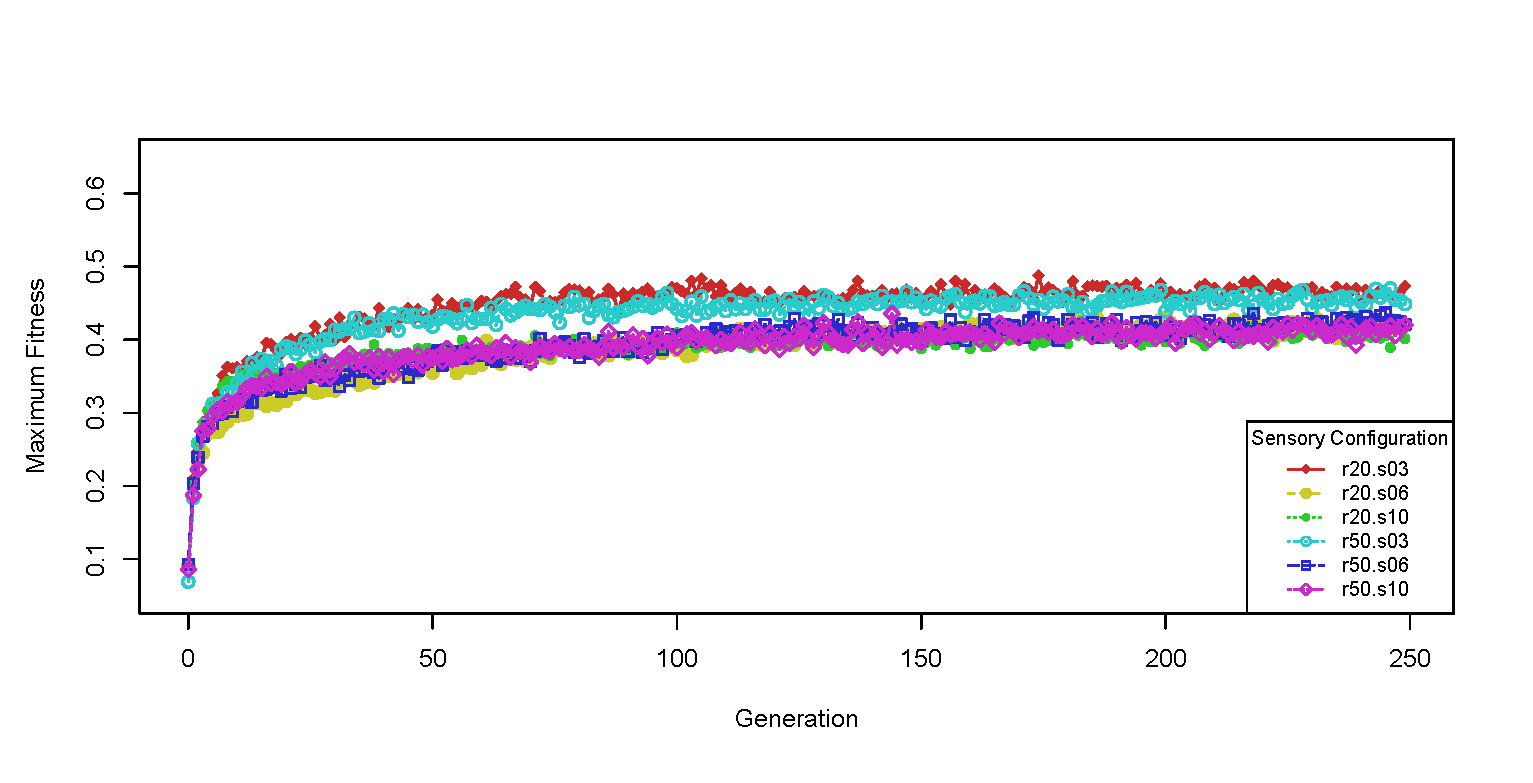
\includegraphics[width=0.80\textwidth]{necc_sensor_runs.eps}
    \end{minipage}
    \caption{Progression of best team task performance over the course of controller evolution, averaged over 30 runs.
    Red and blue curves at the top correspond to teams using three sensors, and yield a higher average task
    performance (with statistical significance), compared to the other sensory configurations tested.}
    \label{fig:runs}
\end{figure*}

\hlcyan{Figures } \ref{fig:evoRuns_Lev1},\ref{fig:evoRuns_Lev2} and \ref{fig:evoRuns_Lev3} \hlcyan{present the progression of maximum team fitness over the course of the controller evolution for each complexity level respectively. The values were averaged over 20 runs}

Figure \ref{fig:runs} presents the progression of maximum team fitness over the course of controller evolution, averaged over 30 runs.
Whilst figure \ref{fig:results} indicated that teams using three sensors achieved the highest overall fitness, 
figure \ref{fig:runs} indicates that team fitness, for this lower number of sensors, after a steep increase during the first 50
generations, remains relatively constant throughput the rest of the evolutionary run.
This implies that if controller evolution can only be run for relatively few generations, then selecting an appropriate sensory
configuration yields significantly beneficial task performance advantages.

These results are supported by related research \cite{SchultzBugajska2003}
that similarly demonstrates a minimal number of sensors and an appropriate sensory configuration leads to desired task performance, 
and increasing the complexity of the sensory configuration does not necessarily result in increased task performance.

This study's research objective was to find a minimal morphology (sensory configuration) such that a morphologically and
behaviorally homogenous team evolve effective collective construction behaviors.
The results are relevant to the larger fields of ER \cite{NolfiFloreano2000} and swarm robotics \cite{Beni2004}
that aim to minimize cost, weight and power requirements of robots.
Another goal of these research fields is to synthesize problem solving collective behaviors that
can be efficiently evolved either \textit{a priori} in simulation and then transferred to counterpart physical robots
\cite{Koosetal2010}, \cite{ZagalRuiz-Del-Solar2007}, \cite{HartlandBredeche2006}
or evolved in real time as the robots interact with their environment \cite{Baele-etal-2009},
\cite{EibenKarafotiasHaasdijk2010}.  This research aims to address future applications of the former approach.

This study deviated from related research that co-evolves both morphology and behavior.
Such approaches let a given artificial evolution process search a space of defined behaviors and morphologies in order to derive 
a sensory-motor configuration and coupled controller that is suited to solving a given task in a given environment
\cite{Sims1994}, \cite{LundLee1997}, \cite{AdamatzkyUlatowski2000}, \cite{MautnerBelew2000}, \cite{LipsonPollack2000},
\cite{HornbyPollack2001}, \cite{HornbyPollack2001b}, \cite{Eggenberger1997}, \cite{BongardPfeifer2003},
\cite{AuerbachBongard2010}, \cite{CheneyLipson2013}, \cite{BuasonZiemke2003}, \cite{BuasonBergfeldtZiemke2005}, 
\cite{AuerbachBongard2014}. 

\hlcyan{In this study, the goal was to determine the ability of HyperNEAT evolved controllers to complete the collective construction task across a variety of different sensory configurations}

\hl{In this study the goal was for the experimenter to design and test a range of morphologies and then have a 
neuro-evolution process evolve an appropriate ANN controller.}
The motivation for this approach was the desire to find a minimal sensory configuration
such that solutions to a collective behavior task are efficiently evolved.  
This falls in line with ER and swarm robotic research objectives of designing swarm robotic systems able to accomplish collective behavior tasks
with minimal cost, weight (number sensors) and power requirements, where the problem solving collective behaviors  
of such robotic systems can be efficiently evolved in minimal time.  

In related research that co-evolves behavior and morphology, especially that dealing with robot teams, there 
is a significant computational and time expense involved.
That is, invariably large behavioral and morphological spaces must be searched and a huge number of possible 
behavior-morphology interactions that must be tested and evaluated.
This research demonstrated that in collective behavior tasks where experimenters have some \textit{a priori} 
knowledge from previous experiments \cite{NitschkeSaEC2012} to guide morphological design, then a limited 
set of exploratory experiments that test a range of morphologies is sufficient (section \ref{subsec:expDesign}). 
Furthermore, methods that co-evolve behavior and morphology must often place significant constraints on the 
types of behaviors and morphologies that can be evolved in order to reduce the size of the search spaces
and the number of behavior-morphology combinations that must be tested and evaluated.  In such a case,
morphological design by the experimenter, and then evolving controllers for these morphologies, is often 
just as effective as the behavior-morphology co-evolution approaches.

In this research the collective construction task 
was more akin to widely studied collective gathering tasks \cite{BonabeauDorigo1998} 
that require agents (robots) to search an environment for resources, and then transport these gathered resources to a home area.  
In this case there was no specific home area, rather the
first gathered block could be connected to any other, 
and then this initial structure became the focal point where all gathered blocks
were transported to.  
Also, the task was made more complex via requiring cooperation (two robots) to move half of the blocks.
Thus cooperative behavior and division of labor was mandated for the team to achieve optimal task performance.  
That is, if all blocks were to be gathered, teams had to effectively split into those that gathered \textit{type A} 
blocks (one robot only) and those that gathered \textit{type B} blocks (two robots needed).
Experimental results achieved on average a maximum of approximately 60 percent of optimal team task performance (figure \ref{fig:results}).
This was a result of limiting the team lifetime duration (table \ref{tab:simParameters}) to lower computational expense,
and the lack of sensors to detect fellow robots.  Both were in the interest of satisfying the research objective, and having purely stigmergic
interactions between robots \cite{BeckersHollandDeneubourg1994}.

The inclusion of sensors for discriminating between team mates and resources in the environment has been demonstrated as
beneficial in collective gathering and construction tasks \cite{NitschkeSaEC2012} and will thus potentially form a part
of future work that aims to test the impact of various morphologies (sensory configurations) 
as collective behavior task complexity increases.  
Specifically, future work will focus on testing
a range of morphologically and behaviorally homogenous and heterogenous teams for varying degrees of complexity of a
collective gathering and construction task.  Increasing complexity in such a task entails having more block types,
where each type requires a different degree of cooperation between robots to move, as well as testing a range of
construction schemas.  Construction schemas dictate the sequence and number of each block type that must be connected
together in order for a structure to be built.  Task difficulty can be regulated via the
construction schema requiring that relatively scare block types be the first building blocks used in construction
\cite{NitschkeSaEC2012}.
% implications of these results are that the amount of time spent running simulations can be greatly reduced.
%This can reduce the time needed to test other parameters, as during a simulation evaluating the ANN at each time step for every agent can take a significant amount of processing time, which is a combinatorial function of the number of nodes in each layer.
%In addition, real world implementations of such a task would be significantly cheaper with less sensors to attach.
%This process can therefore be repeated for other types of multi-agent neuro-evolution tasks, to test during simulation how best to physically design agent implementations.
%This technique can likely be applied to many other neuro-evolutionary tasks involving agent controller design. 
%While it does increase the number of parameters to %optimise -- which may already be fairly large -- the effects may be apparent early and (as shown here) may improve the speed at which future experiments can be run.
%Whilst there has been a significant amount of work in ER that focuses on the co-evolution of behaviour and morphology
%
%With this approach body plans and control policies uniquely suited for
%a machine�s task environment may be found.  However, there has been relatively little work on comparative studies of generative NE methods
%in the context of simulated cooperative multi-robot systems.  The objective of such studies is to ascertain the most appropriate NE
%in order that the behaviors and morphologies of individual robots are co-adapted so as the robots effectively operate in a range of
%collective behaviour task environments.
%This paper focuses only on one subtask of collective construction -- the gathering of blocks by agents --
%as it focuses on the configuration of sensors, although future work will extend this to the full task.
%\section{Future Work}
%This paper focused only on gathering component of the collective construction task. It is currently being extended to the full task by evolving separate controllers for each stage of the construction. The task can also be separated in multiple ways. One division is gathering (as shown here) and construction (placing the gathered blocks in the optimal locations), but the construction task can be done either in two parallel parts by deciding on an optimal structural design and separately evolving a controller which attempts to achieve the evolved design, or it can be merged into one stage by having heuristic-based rewards during placement of gathered blocks to guide evolution towards desirable properties of the target structure.


\section{Conclusions}

This research presented a study on the impact of different robot sensory
configurations (morphologies) on evolving team behaviors in a robot team that 
had to accomplish a collective construction task.  
The collective construction task required cooperation in order
for the team to optimally accomplish it.  The team was behaviorally
and morphological homogenous where the morphology was determined \textit{a priori}
by the experimenter and an accompanying ANN controller was evolved.
The research objective was to investigate what degree of morphological complexity 
would be amenable to the efficient evolution of effective collective behaviors.
This objective addresses future ER goals of designing robot swarms that have minimal cost,
power and weight requirements, where problem solving collective behaviors must be 
efficiently evolved. 
Results indicate that minimal sensory configurations yield the
highest task performance, and that effective collective behaviors can be more
efficiently evolved for such minimal morphologies.  
In this collective construction task, increasing morphological complexity did 
not result in increased task performance over minimal morphology-behavior couplings.
%would yield task performance benefits
%over more complex morphologies.


%A multi-agent gathering task was investigated, using the HyperNEAT neuro-evolutionary method to generate partially pre-designed controllers for simplistic autonomous robots. Various configurations of both number of sensors and sensor ranges were tested, to see if the layout of sensory input could have an effect on task performance. It was found that while sensor range was largely irrelevant in this task, reducing the number of sensors improved performance both significantly and consistently across even low numbers of generations -- a result which has implications for not only simulations, but possible future physical implementations of similar tasks.

\bibliographystyle{IEEEtran}
\bibliography{IEEEabrv,necc_paper,EvoComp,Dissertation}









\end{document} 